\documentclass{standalone}
\usepackage{tikz}
\usetikzlibrary{automata, positioning, arrows}

\begin{document}
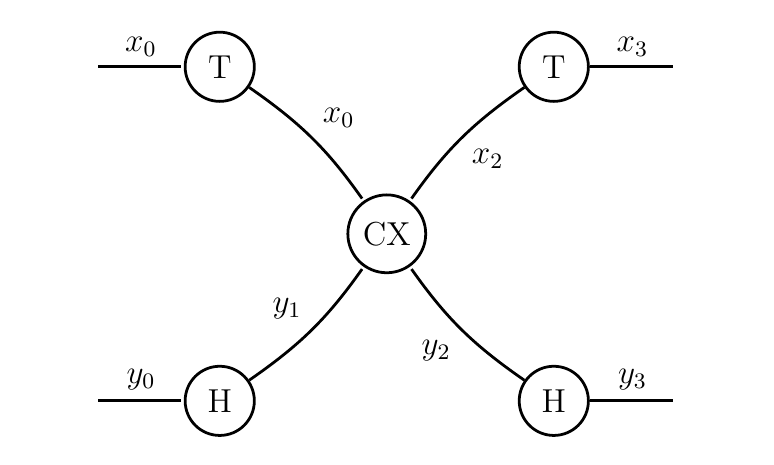
\begin{tikzpicture}[shorten >=1pt,node distance=3cm,on grid,auto,line width=1pt, every edge/.style={draw, -},every node/.style={font=\large}]

  \node[state] (c0) {CX};
  \node[state] (s1) [above left=of c0] {T};
  \node[state, draw=none] (n1) [left=2cm of s1] {};

  \node[state] (s2) [above right=of c0] {T};
  \node[state, draw=none] (n2) [right=2cm of s2] {};

  \node[state] (s3) [below left=of c0] {H};
  \node[state, draw=none] (n3) [left=2cm of s3] {};

  \node[state] (s4) [below right=of c0] {H};
  \node[state, draw=none] (n4) [right=2cm of s4] {};


  \path[-] 
        (n1) edge node {$x_0$} (s1)
        (s2) edge node {$x_3$} (n2)
        (n3) edge node {$y_0$} (s3)
        (s4) edge node {$y_3$} (n4)
        (s1) edge[bend left=10] node {$x_0$} (c0)
        (s2) edge[bend right=10] node {$x_2$} (c0)
        (s3) edge[bend right=10] node {$y_1$} (c0)
        (s4) edge[bend left=10] node {$y_2$} (c0);
\end{tikzpicture}
\end{document}